\documentclass{article}
\usepackage[utf8]{inputenc}
% are all of these packages really necessary?
% no.
% i'm just too lazy to only grab the packages i want for a specific
% document, so i just glob all of my most commonly used packages together
% this is bad practice.
\usepackage{amsmath,amsthm,amssymb,amsfonts, fancyhdr, color, comment, graphicx, environ, mdframed, soul, calc, enumitem, mdframed, xcolor, geometry, empheq, mathtools, tikz, pgfplots, caption, subcaption, hyperref}

\usetikzlibrary{external}
\tikzexternalize[prefix=tikz/,optimize command away=\includepdf]

%tikzpicture
\usepackage{tikz}
\usepackage{scalerel}
\usepackage{pict2e}
\usepackage{tkz-euclide}
\usetikzlibrary{calc}
\usetikzlibrary{patterns,arrows.meta}
\usetikzlibrary{shadows}
\usetikzlibrary{external}

%pgfplots
\usepackage{pgfplots}
\pgfplotsset{compat=newest}
\usepgfplotslibrary{statistics}
\usepgfplotslibrary{fillbetween}
\usepgfplotslibrary{polar}

\tikzset{external/export=true}
\pgfplotsset{
    standard/.style={
    axis line style = thick,
    trig format=rad,
    enlargelimits,
    axis x line=middle,
    axis y line=middle,
    enlarge x limits=0.15,
    enlarge y limits=0.15,
    every axis x label/.style={at={(current axis.right of origin)},anchor=north west},
    every axis y label/.style={at={(current axis.above origin)},anchor=south east}
    }
}
\newcommand*\widefbox[1]{\fbox{\hspace{2em}#1\hspace{2em}}}
% Command "alignedbox{}{}" for a box within an align environment
% Source: http://www.latex-community.org/forum/viewtopic.php?f=46&t=8144
\newlength\dlf  % Define a new measure, dlf
\newcommand\alignedbox[2]{
% Argument #1 = before & if there were no box (lhs)
% Argument #2 = after & if there were no box (rhs)
&  % Alignment sign of the line
{
\settowidth\dlf{$\displaystyle #1$}  
    % The width of \dlf is the width of the lhs, with a displaystyle font
\addtolength\dlf{\fboxsep+\fboxrule}  
    % Add to it the distance to the box, and the width of the line of the box
\hspace{-\dlf}  
    % Move everything dlf units to the left, so that & #1 #2 is aligned under #1 & #2
\boxed{#1 #2}
    % Put a box around lhs and rhs
}
}

\hypersetup{
    colorlinks=true,
    linkcolor=blue,
    filecolor=magenta,      
    urlcolor=cyan,
    pdftitle={Midterm 2 Review Solutions},
    pdfpagemode=UseOutlines,
    bookmarksopen=true,
    pdfauthor={Christina Phan}
}
\newcommand{\lrp}[1]{\left( #1 \right)}
\newcommand{\abs}[1]{\left\vert #1 \right\vert}
\newcommand{\lra}[1]{\left\langle #1 \right\rangle}
\newcommand{\lrb}[1]{\left[ #1 \right]}
\newcommand{\norm}[1]{\left\lVert #1 \right\rVert}
\newcommand{\iintR}[0]{\iint\limits_{R}}
\renewcommand{\u}[0]{\mathbf{u}}
\renewcommand{\i}[0]{\mathbf{i}}
\renewcommand{\j}[0]{\mathbf{j}}
\renewcommand{\k}[0]{\mathbf{k}}
\newcommand{\T}[0]{\mathbf{T}}
\newcommand{\N}[0]{\mathbf{N}}
\newcommand{\B}[0]{\mathbf{B}}
\renewcommand{\r}[0]{\mathbf{r}}
\renewcommand{\a}[0]{\mathbf{a}}
\renewcommand{\v}[0]{\mathbf{v}}
\newcommand{\F}[0]{\mathbf{F}}
\newcommand{\eqq}[0]{\stackrel{?}{=}}

\renewcommand{\arraystretch}{1.25}

\geometry{letterpaper, portrait, margin=1in}
\renewcommand{\footrulewidth}{0.8pt}
\setlength\parindent{0pt}
\pagestyle{fancy}
\lhead{Christina Phan}
\rhead{MAT 21D} 
\chead{\textbf{Midterm 2 Review Solutions}}

\newcommand{\Solution}{\textit{Solution}}
\pgfplotsset{compat=1.18}
\begin{document}

\phantomsection
\addcontentsline{toc}{section}{Problem 1}\textbf{Problem 1}

Find the point on the curve $y=e^x$ where the curvature is greatest.

\Solution

Recall that the curvature of any function at the point $x$ is given by \begin{equation*}
    \kappa (x)=\frac{\left|f''(x)\right|}{(1+f'(x)^2)^{3/2}}
\end{equation*}
(Homework 9, 2(a); Campuswire \#45)

If $y=e^x$, then
\begin{align*}
    y'(x)&=e^x\\
    y''(x)&=e^{x}
\end{align*}
Therefore, the curvature at the point $x$ for the function $y=e^x$ is
\begin{equation*}
    \kappa(x)=\frac{\left|e^x\right|}{\lrp{1+\lrp{e^x}^2}^{3/2}}=\frac{e^x}{\lrp{(1+e^{2x}}^{3/2}}=e^x\lrp{1+e^{2x}}^{-3/2}\tag{$e^x>0$ for all $x$}
\end{equation*}
Recall back from Calculus 1 (MAT 21A) that the maximum value of $\kappa(x)$ occurs when $\kappa'(x)>0$ for all $x<c$ and $\kappa'(x)<0$ for all $x>c$.

Let's find $\kappa'(x)$.
\begin{align*}
    \kappa'(x)&=e^x\lrp{1+e^{2x}}^{-3/2}+\lrp{-\frac{3}{2}\lrp{1+e^{2x}}^{-5/2}\lrp{2e^{2x}}}e^x\\
    &=e^x\lrp{1+e^{2x}}^{-3/2}-3\lrp{1+e^{2x}}^{-5/2}e^{3x}\\
    &=\lrp{e^x}\lrp{1+e^{2x}}^{-5/2}\lrp{\lrp{1+e^{2x}}-3e^{2x}}\tag{factor}\\
    &=\lrp{e^x}\lrp{1+e^{2x}}^{-5/2}\lrp{1-2e^{2x}}
\end{align*}
We know $(e^x)$ and $\displaystyle \lrp{1+e^{2x}}^{-5/2}$ are only going to give us positive values (since $e^x>0$ for all $x$), so $\lrp{-2e^{2x}}$ is our only hope in finding a critical points and determining our maximum curvature $x$-value.
\begin{align*}
    \lrp{e^x}\lrp{1+e^{2x}}^{-5/2}\lrp{1-2e^{2x}}&=0\\
    \lrp{1-2e^{2x}}&=\tag{$(e^x)$ and $\lrp{1+e^{2x}}^{-5/2}$ never equal $0$}\\
    -2e^{2x}&=-1\\
    e^{2x}&=\frac{1}{2}\\
    2x&=\ln\frac{1}{2}\tag{$\ln e^{2x}=2x$}\\
    x&=\frac{1}{2}\ln\frac{1}{2}\\
    &=\ln \frac{1}{\sqrt{2}}\tag{$\frac{1}{2}\ln\frac{1}{2}=\ln \lrp{\frac{1}{2}}^{1/2}=\ln \frac{1}{2^{1/2}}$}
\end{align*}
Let's draw out our good old number line to see the behavior of $\kappa'(x)$.

When $x=-1$,
\begin{align*}
    \kappa'(-1)=\lrp{e^{-1}}\lrp{1+e^{2(-1)}}^{-5/2}\lrp{1-2e^{2(-1)}}=\lrp{\frac{1}{e}}\lrp{1+\frac{1}{e^2}}^{-5/2}\lrp{1-\frac{2}{e^2}}>0\tag{all positives}
\end{align*}
When $x = 0$,
\begin{align*}
    \kappa'(0)&=\lrp{e^0}\lrp{1+e^{2(0)}}^{-5/2}\lrp{1-2e^{2(0)}}=\lrp{1}\lrp{1+1}^{-5/2}\lrp{1-2}=\lrp{1}\lrp{2}^{-5/2}\lrp{-1}<0\tag{one negative}
\end{align*}


\tikzset{every picture/.style={line width=0.75pt}} %set default line width to 0.75pt        
\begin{center}
  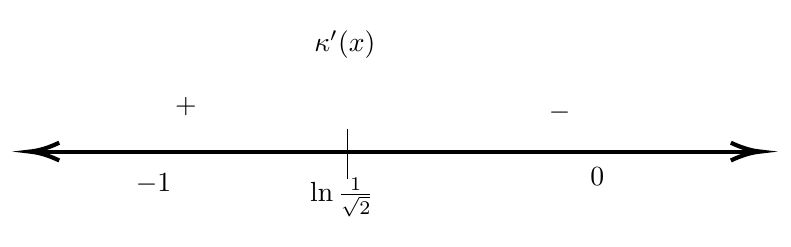
\begin{tikzpicture}[x=0.75pt,y=0.75pt,yscale=-1,xscale=1]
%uncomment if require: \path (0,300); %set diagram left start at 0, and has height of 300

%Straight Lines [id:da6895024679986879] 
\draw [line width=1.5]    (136.17,169.83) -- (482.17,169.83) ;
\draw [shift={(485.17,169.83)}, rotate = 180] [color={rgb, 255:red, 0; green, 0; blue, 0 }  ][line width=1.5]    (14.21,-4.28) .. controls (9.04,-1.82) and (4.3,-0.39) .. (0,0) .. controls (4.3,0.39) and (9.04,1.82) .. (14.21,4.28)   ;
\draw [shift={(133.17,169.83)}, rotate = 0] [color={rgb, 255:red, 0; green, 0; blue, 0 }  ][line width=1.5]    (14.21,-4.28) .. controls (9.04,-1.82) and (4.3,-0.39) .. (0,0) .. controls (4.3,0.39) and (9.04,1.82) .. (14.21,4.28)   ;
%Straight Lines [id:da062314200534874464] 
\draw    (286.17,158.83) -- (286.17,182.83) ;

% Text Node
\draw (269,110.4) node [anchor=north west][inner sep=0.75pt]    {$\kappa '( x)$};
% Text Node
\draw (267,181.4) node [anchor=north west][inner sep=0.75pt]    {$\ln\frac{1}{\sqrt{2}}$};
% Text Node
\draw (402,176.4) node [anchor=north west][inner sep=0.75pt]    {$0$};
% Text Node
\draw (183,179.4) node [anchor=north west][inner sep=0.75pt]    {$-1$};
% Text Node
\draw (202,142.4) node [anchor=north west][inner sep=0.75pt]    {$+$};
% Text Node
\draw (382,145.4) node [anchor=north west][inner sep=0.75pt]    {$-$};


\end{tikzpicture}  
\end{center}


Since $\kappa'(x)>0$ when $x < \ln \dfrac{1}{\sqrt{2}}$ and $\kappa'(x)<0$ when $x > \ln\dfrac{1}{\sqrt{2}}$, the absolute maximum of $\kappa(x)$ occurs at $x=\ln\dfrac{1}{\sqrt{2}}$.

At $x=\ln\dfrac{1}{\sqrt{2}}$,
\begin{equation*}
    y\lrp{\ln\dfrac{1}{\sqrt{2}}}=e^{\ln\dfrac{1}{\sqrt{2}}}=\frac{1}{\sqrt{2}}\tag{$e$ and $\ln$ ``cancel"}
\end{equation*}
Therefore the curvature is greatest at 
\begin{equation*}
    \boxed{\lrp{\ln\dfrac{1}{\sqrt{2}},\dfrac{1}{\sqrt{2}}}}
\end{equation*}
\phantomsection
\addcontentsline{toc}{section}{Problem 2}\textbf{Problem 2}

Find the length of the curve $\r(t)=\lra{3\cos t, 3\sin t, 2t^{3/2}}$, $0\leq t\leq 3$.

\Solution

Recall that the arc length parameter from $t_0$ to $t$ is
\begin{equation*}
    s(t)=\int_{t_0}^t\norm{\r'(\tau)}\,d\tau
\end{equation*}
Let's find $\r'(t)$, $\norm{\r'(t)}$, and $s(t)$.
\begin{align*}
    \r'(t)&=\lra{-3\sin t,3\cos t, 3t^{1/2}}\\
    \norm{\r'(t)}&=\sqrt{(-3\sin t)^2+(3\cos t)^2 +\lrp{3t^{1/2}}^2}\\
    &=\sqrt{9\sin^2 t+9\cos^2t+9t}\\
    &=\sqrt{9\lrp{\sin^2 t +\cos^2 t}+9t}\\
    &=\sqrt{9+9t}\tag{$\sin^2t+\cos^2t=1$}\\
    &=\sqrt{9(1+t)}\\
    &=3\sqrt{1+t}\\
    s(t)&=\int_0^t 3\sqrt{1+t}\,d\tau\tag{we know $0\leq t\leq 3$, so let $t_0=0$}
\end{align*}
If $\displaystyle s(t)=\int_0^t3\sqrt{1+t}\,d\tau$ where $t_0=0$, then the length of the curve from $t=0$ to $t=3$ is
\begin{align*}
    s(3)&=\int_0^3 3\sqrt{1+\tau}\,d\tau\\
    &=3\int_0^3 (1+\tau)^{1/2}\,d\tau\tag{we can take constants out}\\
    &=3\lrb{\frac{2}{3}(1+\tau)^{3/2}}_0^3\\
    &=3\lrp{\lrp{\frac{2}{3}(1+3)^{3/2}}-\lrp{\frac{2}{3}(1+0)^{3/2}}}\\
    &=3\lrp{\lrp{\frac{2}{3}(4)^{3/2}}-\lrp{\frac{2}{3}}}\\
    &=3\lrp{\frac{2}{3}(8)-\frac{2}{3}}\tag{$4^{3/2}=\lrp{4^{1/2}}^3=\lrp{2}^3=8$}\\
    &=3\lrp{\frac{14}{3}}\\
    &=\boxed{14}
\end{align*}
\phantomsection
\addcontentsline{toc}{section}{Problem 3}\textbf{Problem 3}

Find $\T$, $\N$, $\B$ and $\kappa$ as functions of $t$ for $\r(t)\lra{\sin t, \sqrt{2}\cos t, \sin t}$.

\Solution

Recall that $\T$, $\N$, $\B$ , and $\kappa$ are
\begin{align*}
    \T&=\frac{\r'(t)}{\lVert \r'(t)\rVert}\\
    \N&=\frac{\T'(t)}{\lVert \T'(t)\rVert}\\
    \B&=\T\times \N\\
    \kappa&=\frac{\lVert \T'(t)\rVert}{\lVert \r'(t)\rVert}
\end{align*}
Let's find $\T$, $\N$, $\B$, and $\kappa$ for this problem.
\begin{align*}
    \r'(t)&=\lra{\cos t, -\sqrt{2}\sin t,\cos t}\\
    \norm{\r'(t)}&=\sqrt{\cos^2 t + \lrp{-\sqrt{2}\sin t}^2+\cos^2t}\\
    &=\sqrt{\cos ^2 t + 2\sin^2 t+\cos^2t}\\
    &=\sqrt{2\cos^2 t+2\sin^2 t}\\
    &=\sqrt{2\lrp{\cos^2 t+\sin^2 t}}\\
    &=\sqrt{2}\tag{$\cos^2 t+\sin^2 t =1$}\\
    \T&=\frac{1}{\sqrt{2}}\lra{\cos t, -\sqrt{2}\sin t,\cos t}=\lra{\frac{\cos t}{\sqrt{2}},-\sin t,\frac{\cos t}{\sqrt{2}}}\\
    \T'(t)&=\lra{-\frac{\sin t}{\sqrt{2}}, -\cos t,-\frac{\sin t}{\sqrt{2}}}\\
    \norm{\T'(t)}&=\sqrt{\lrp{-\frac{\sin t}{\sqrt{2}}}^2+\lrp{-\cos t}^2+\lrp{-\frac{\sin t}{\sqrt{2}}}^2}\\
    &=\sqrt{\frac{\sin^2 t}{2}+\cos ^2 t+\frac{\sin ^2 t}{2}}\\
    &=\sqrt{\sin^2 t+\cos ^2 t}\\
    &=\sqrt{1}\tag{$\sin^2 t+\cos ^2 t=1$}\\
    &=1\\
    \N&=\frac{1}{1}\lra{-\frac{\sin t}{\sqrt{2}}, -\cos t,-\frac{\sin t}{\sqrt{2}}}=\lra{-\frac{\sin t}{\sqrt{2}}, -\cos t,-\frac{\sin t}{\sqrt{2}}}\\
    \B&=\lra{\frac{\cos t}{\sqrt{2}},-\sin t,\frac{\cos t}{\sqrt{2}}}\times \lra{-\frac{\sin t}{\sqrt{2}}, -\cos t,-\frac{\sin t}{\sqrt{2}}}\\
    &=\begin{vmatrix}
    \i & \j & \k\\
    \frac{\cos t}{\sqrt{2}} & -\sin t & \frac{\cos t}{\sqrt{2}}\\
    -\frac{\sin t}{\sqrt{2}} & -\cos t & -\frac{\sin t}{\sqrt{2}}
    \end{vmatrix}\\
    &=\lrp{\frac{\sin^2 t}{\sqrt{2}}+\frac{\cos ^2 t}{\sqrt{2}}}\i -\lrp{-\frac{\sin t\cos t}{2}+\frac{\sin t\cos t}{2}}\j + \lrp{-\frac{\cos ^2 t}{\sqrt{2}}-\frac{\sin^2 t}{\sqrt{2}}}\k\\
    &=\lrp{\frac{1}{\sqrt{2}}\lrp{\sin^2 t+\cos ^2 t}}\i-\lrp{0}\j + \lrp{-\frac{1}{\sqrt{2}}\lrp{\cos^2 t+\sin^2 t}}\k\\
    &=\lrp{\frac{1}{\sqrt{2}}}\i-\lrp{0}\j +\lrp{-\frac{1}{\sqrt{2}}}\k\tag{$\sin^2 t+\cos^2t=1$}\\
    &=\lra{\frac{1}{\sqrt{2}},0,-\frac{1}{\sqrt{2}}}\\
    \kappa&=\frac{1}{\sqrt{2}}
\end{align*}
Our final answer is
\begin{subequations}
    \begin{empheq}[box=\widefbox]{align}
        \T&=\lra{\frac{\cos t}{\sqrt{2}},-\sin t,\frac{\cos t}{\sqrt{2}}}\nonumber\\
        \N&=\lra{-\frac{\sin t}{\sqrt{2}},-\cos t,-\frac{\sin t}{\sqrt{2}}}\nonumber\\
        \B&=\lra{\frac{1}{\sqrt{2}},0,-\frac{1}{\sqrt{2}}}\nonumber\\
        \kappa&=\frac{1}{\sqrt{2}}\nonumber
    \end{empheq}
\end{subequations}
\phantomsection
\addcontentsline{toc}{section}{Problem 4}\textbf{Problem 4}

Integrate $f(x,y,z)=2x-3y^2-2z+3$ over the line segment from the origin to $(1,1,1)$ and over the line segments from the origin to $(1,1,0)$ and from $(1,1,0)$ to $(1,1,1)$.

\Solution

\phantomsection
\addcontentsline{toc}{subsection}{Origin To (1,1,1)}\textbf{Origin To $(1,1,1)$}

Let's find $\r(t)$ from the origin $(0,0,0)$ to the point $(1,1,1)$.
\begin{align*}
    \r(t)&=\lra{0,0,0}+\lra{1-0,1-0,1-0}t=\lra{0,0,0}+\lra{t,t,t}=\lra{t,t,t}\tag{$0\leq t \leq 1$}
\end{align*}
We know $0\leq t\leq 1$ since at $t=0$, $\r(0)=\lra{0,0,0}$, and at $t=1$, $\r(1)=\lra{1,1,1}$.

If $\r(t)=\lra{t,t,t}$, then
\begin{align*}
    f\lrp{\r(t)}&=2t-3t^2-2t+3=-3t^2+3\\
    \r'(t)&=\lra{1,1,1}\\
    \norm{\r'(t)}&=\sqrt{1^2+1^2+1^2}=\sqrt{3}
\end{align*}
Let's evaluate the integral.
\begin{align*}
    \int_C 2x-3y^2-2z+3\,ds&=\int_0^1\lrp{-3t^2+3}\lrp{\sqrt{3}}\,dt\\
    &=\sqrt{3}\int_0^1 -3t^2+3\,dt\tag{we can take constants out}\\
    &=\sqrt{3}\lrb{-t^3+3t}_0^1\\
    &=\sqrt{3}\lrp{-1+3}\\
    &=\boxed{2\sqrt{3}}
\end{align*}

\phantomsection
\addcontentsline{toc}{subsection}{Origin To (1,1,0) and (1,1,0) to (1,1,1)}\textbf{Origin To $(1,1,0)$ and $(1,1,0)$ to $(1,1,1)$}

We're going to need two $\r(t)$'s (two curves), one for the origin $(0,0,0)$ to the point $(1,1,0)$ and another for the point $(1,1,0)$ to the point $(1,1,1)$.

Let $\r_1(t)$ be the path from the origin $(0,0,0)$ to the point $(1,1,0)$.
\begin{align*}
    \r_1(t)&=\lra{0,0,0}+\lra{1-0,1-0,0-0}t=\lra{0,0,0}+\lra{t,t,0}=\lra{t,t,0}\tag{$0\leq t\leq 1$}
\end{align*}
Let $\r_2(t)$ be the path from the point $(1,1,0)$ to the point $(1,1,1)$.
\begin{align*}
    \r_2(t)&=\lra{1,1,0}+\lra{1-1,1-1,1=0}t=\lra{1,1,0}+\lra{0,0,t}=\lra{1,1,t}\tag{$0\leq t\leq 1$}
\end{align*}
We know that $0\leq t\leq $ are the bounds for both $\r_1(t)$ and $\r_2(t)$ since we get the correct end points at $t=0$ and $t=1$ (test it out yourself $<$3).

If $\r_1(t)=\lra{t,t,0}$, then
\begin{align*}
    \r'_1(t)&=\lra{1,1,0}\\
    \norm{\r'_1(t)}&=\sqrt{1^2+1^2+0^2}=\sqrt{2}
\end{align*}
If $\r_2(t)=\lra{1,1,t}$, then
\begin{align*}
    \r'_2(t)&=\lra{0,0,1}\\
    \norm{\r'_2(t)}&=\sqrt{0^2+0^2+1^2}=\sqrt{1}=1
\end{align*}
Let's evaluate the integral(s).
\begin{align*}
    \int_C 2x-3y^2-2z+3\,ds&=\underbrace{\int_{C_1}2x-3y^2-2z+3\,ds}_{\r_1(t)}+\underbrace{\int_{C_2}2x-3y^2-2z+3\,ds}_{\r_2(t)}\\
    &=\int_0^1 \Big(2t-3t^2-2(0)+3\Big)\lrp{\sqrt{2}}\,dt+\int_0^1 \Big(2(1)-3(1)^2-2t+3\Big)\lrp{1}\,dt\\
    &=\sqrt{2}\int_0^1 2t-3t^2+3\,dt+\int_0^1 2-3-2t+3\,dt\tag{we can take constants out}\\
    &=\sqrt{2}\lrb{t^2-t^3+3t}_0^1 + \lrb{2t-3t-t^2+3t}_0^1\\
    &=\sqrt{2}\Big(1^2-1^3+3(1)\Big)+\Big(2(1)-3(1)-1^2+3(1)\Big)\\
    &=\sqrt{2}\lrp{3}+\lrp{1}\\
    &=3\sqrt{2}+1
\end{align*}
Our final answer is
\begin{subequations}
    \begin{empheq}[box=\widefbox]{align}
        \text{origin to }(1,1,1)\text{: } &2\sqrt{3}\nonumber\\
        \text{origin to }(1,1,0)\text{ and then to }(1,1,1)\text{: }&3\sqrt{2}+1\nonumber
    \end{empheq}
\end{subequations}
\phantomsection
\addcontentsline{toc}{section}{Problem 5}\textbf{Problem 5} 

Integrate $f(x,y,z)=\sqrt{x^2+z^2}$ over the circle $\r(t)=\lra{0,a\cos t,a\sin t}$, $0\leq t\leq 2\pi$.

\Solution

If $\r(t)=\lra{0,a\cos t,a\sin t}$, then
\begin{align*}
    \r'(t)&=\lra{0,-a\sin t, a\cos t}\\
    \norm{\r'(t)}&=\sqrt{0^2 + \lrp{-a\sin t}^2 +\lrp{a \cos t}^2}\\
    &=\sqrt{a^2\sin ^2 t+a^2\cos ^2 t}\\
    &=\sqrt{a^2\lrp{\sin ^2 t+\cos ^2 t}}\\
    &=\sqrt{a^2}\tag{$\sin ^2 t+\cos ^2 t=1$}\\
    &=a\tag{not $\left|a\right|$ since $a$ is radius of circle}
\end{align*}
Let's evaluate the integral.
\begin{align*}
    \int_C f(x,y,z)\,ds&=\int_C \sqrt{x^2+z^2}\,ds\\
    &=\int_0^{2\pi}\lrp{\sqrt{0^2+\lrp{a\sin t)^2}}}\lrp{a}\,dt\\
    &=\int_0^{2\pi}a\sqrt{a^2\sin^2 t}\,dt\\
    &=\int_0^{2\pi}a\lrp{a\left|\sin t\right|}\,dt\\
    &= \int_0^{\pi}a\lrp{a\sin t}\,dt+\int_{\pi}^{2\pi}a\lrp{-a\sin t}\,dt\tag{$\sin t\geq0$ when $0\leq t\leq \pi$, $\sin t\leq0$ when $\pi \leq t\leq 2\pi$}\\
    &=\int_0^\pi a^2\sin t\,dt+\int_{\pi}^{2\pi}-a^2\sin t\,dt\\
    &=\lrb{-a^2\cos t}_0^{\pi}+\lrb{a^2\cos t}_{\pi}^{2\pi}\\
    &=\Big(-a^2\cos \pi-\lrp{-a^2\cos 0}\Big)+\lrp{a^2\cos 2\pi -a^2\cos \pi}\\
    &=\Big(-a^2\lrp{-1}+a^2\lrp{1}\big)+\Big(a^2(1)-a^2(-1)\Big)\\
    &=\lrp{2a^2}+\lrp{2a^2}\\
    &=\boxed{4a^2}
\end{align*}

\phantomsection
\addcontentsline{toc}{section}{Problem 6}\textbf{Problem 6}

Evaluate the integral $\displaystyle \int_{(1,1,1)}^{(10,3,3)}\,dx-\sqrt{\frac{z}{y}}\,dy-\sqrt{\frac{y}{z}}\,dz$.

\Solution

Let $\displaystyle\F(x,y,z)=\lra{1,-\sqrt{\frac{z}{y}},-\sqrt{\frac{y}{z}}}$. 

If we can prove that $\F$ is conservative, then there exists an $f$ such that $\F=\nabla f$.

If $\F$ is conservative, then by the ``component test",
\begin{align*}
    \frac{\partial M}{\partial y}=\frac{\partial N}{\partial x},\hspace{2em}\frac{\partial M}{\partial z}=\frac{\partial P}{\partial x},\hspace{2em} \text{and}\hspace{2em}\frac{\partial N}{\partial z}=\frac{\partial P}{\partial y}.
\end{align*}
Let's check if $\F$ is conservative.

\phantomsection
\addcontentsline{toc}{subsection}{M and N}
For $\displaystyle \frac{\partial M}{\partial y}$ and $\displaystyle \frac{\partial N}{\partial x}$,
\begin{align*}
    \frac{\partial M}{\partial y}&=0\\
    \frac{\partial N}{\partial x}&=0
\end{align*}
Therefore, $\displaystyle \frac{\partial M}{\partial y}=0=\displaystyle \frac{\partial N}{\partial x}$.

\phantomsection
\addcontentsline{toc}{subsection}{M and P}
For $\displaystyle \frac{\partial M}{\partial z}$ and $\displaystyle\frac{\partial P}{\partial x}$,
\begin{align*}
    \frac{\partial M}{\partial z}&=0\\
    \frac{\partial P}{\partial x}&=0
\end{align*}
Therefore, $\displaystyle \frac{\partial M}{\partial z}=0=\displaystyle\frac{\partial P}{\partial x}$.

\phantomsection
\addcontentsline{toc}{subsection}{N and P}
For $\displaystyle \frac{\partial N}{\partial z}$ and $\displaystyle\frac{\partial P}{\partial y}$,
\begin{align*}
    \frac{\partial N}{\partial z}&=-\frac{1}{2}\lrp{\frac{z}{y}}^{-1/2}\lrp{\frac{1}{y}}=-\frac{1}{2}\lrp{\frac{y}{z}}^{1/2}\lrp{\frac{1}{y}}=-\frac{1}{2}\lrp{\frac{1}{z^{1/2}y^{1/2}}}=-\frac{1}{2\sqrt{yz}}\\
    \frac{\partial P}{\partial y}&=-\frac{1}{2}\lrp{\frac{y}{z}}^{-1/2}\lrp{\frac{1}{z}}=\frac{1}{2}\lrp{\frac{z}{y}}^{1/2}\lrp{\frac{1}{z}}=-\frac{1}{2}\lrp{\frac{1}{y^{1/2}z^{1/2}}}=-\frac{1}{2\sqrt{yz}}
\end{align*}
Therefore, $\displaystyle \frac{\partial N}{\partial z}=-\frac{1}{2\sqrt{yz}}=\displaystyle\frac{\partial P}{\partial y}$.

Since $\displaystyle \frac{\partial M}{\partial y}=\frac{\partial N}{\partial x}$, $\displaystyle \frac{\partial M}{\partial z}=\frac{\partial P}{\partial x}$, and $\displaystyle \frac{\partial N}{\partial z}=\frac{\partial P}{\partial y}$, $\F$ is conservative.

Let's start finding $f(x,y,z)$ so we can evaluate the integral.


Since $\displaystyle \frac{\partial f}{\partial x}=1$,
\begin{align*}
    f(x,y,z)&=x+g(y,z)
\end{align*}
Since $\displaystyle \frac{\partial f}{\partial y}=-\sqrt{\frac{z}{y}}$,
\begin{align*}
    \frac{\partial f}{\partial y}=0+\frac{\partial g}{\partial y}&=-\sqrt{\frac{z}{y}}\\
    \implies \frac{\partial g}{\partial y}&=-\sqrt{\frac{z}{y}}\\
    \implies f(x,y,z)&=x+\int-\sqrt{\frac{z}{y}}\,dy\\
    &=x-\sqrt{z}\int y^{-1/2}\,dy\tag{we can take constants out}\\
    &=x-\sqrt{z}\lrp{2y^{1/2}}+h(z)\\
    &=x-2\sqrt{yz}+h(z)
\end{align*}
Since $\displaystyle \frac{\partial f}{\partial z}=-\sqrt{\frac{y}{z}}$,
\begin{align*}
    \frac{\partial f}{\partial z}=0-2\lrp{\frac{1}{2\sqrt{yz}}}\lrp{{y}}+\frac{\partial h}{\partial z}&=-\sqrt{\frac{y}{z}}\\
    -\frac{\sqrt{y}}{\sqrt{z}}+\frac{\partial h}{\partial z}&=-\sqrt{\frac{y}{z}}\\
    \implies \frac{\partial h}{\partial z}&=0\\
    \implies f(x,y,z)&=x-2\sqrt{yz}\tag{let $C=0$ aka ignore $C$}
\end{align*}
Since $f(x,y,z)=x-2\sqrt{yz}$ and $\displaystyle \F(x,y,z)=\nabla f$,
\begin{align*}
    \int_{(1,1,1)}^{(10,3,3)}\,dx-\sqrt{\frac{z}{y}}\,dy-\sqrt{\frac{y}{z}}\,dz&=\lrb{f(x,y,z)}_{(1,1,1)}^{(10,3,3)}\\
    &=f(10,3,3)-f(1,1,1)\\
    &=\lrp{10-2\sqrt{(3)(3)}}-\lrp{1-2\sqrt{(1)(1)}}\\
    &=\lrp{10-2\sqrt{9}}-\lrp{1-2\sqrt{1}}\\
    &=\lrp{10-2(3)}-\lrp{1-2(1)}\\
    &=\lrp{4}-\lrp{-1}\\
    &=\boxed{5}
\end{align*}
\textbf{Note}

You could have also guessed and checked what the potential function $f$ is instead of doing the formal method.

\phantomsection
\addcontentsline{toc}{section}{Problem 7}\textbf{Problem 7}

Integrate $\F(x,y,z)=\lra{3x^2y,x^3+1,9z^2}$ around the circle cut by the plane $x=2$ from the sphere $x^2+y^2+z^2=9$.

\Solution

There are two methods to solve this problem. One is a lot more clever and can save you time on an exam, but it might be harder to remember. Let's do both methods.

\phantomsection
\addcontentsline{toc}{subsection}{Conservative Definition Method}\textbf{Conservative Definition Method}

Recall that if $\F$ is conservative, then $\displaystyle\oint_C \F\cdot d\r=0$ for \textbf{every} curve $C$.

In this problem our curve $C$ is the circle cut by the plane $x=2$ from the sphere $x^2+y^2+z^2=9$ (we are going around the entire circle). 

If we can prove that $\F(x,y,z)$ is conservative, then  $\displaystyle\oint_C \F\cdot d\r$ around the circle cut by the plane $x=2$ from the sphere $x^2+y^2+z^2=9$ is equal to $0$.

We can prove that $\F$ is conservative by the ``component test".

Recall that if $\F$ is conservative, then by the ``component test",
\begin{align*}
    \frac{\partial M}{\partial y}=\frac{\partial N}{\partial x},\hspace{2em}\frac{\partial M}{\partial z}=\frac{\partial P}{\partial x},\hspace{2em} \text{and}\hspace{2em}\frac{\partial N}{\partial z}=\frac{\partial P}{\partial y}.
\end{align*}
Let's check if $\F$ is conservative.

\phantomsection
\addcontentsline{toc}{subsubsection}{M and N}
For $\displaystyle \frac{\partial M}{\partial y}$ and $\displaystyle \frac{\partial N}{\partial x}$,
\begin{align*}
    \frac{\partial M}{\partial y}&=3x^2\\
    \frac{\partial N}{\partial x}&=3x^2
\end{align*}
Therefore, $\displaystyle \frac{\partial M}{\partial y}=3x^2=\displaystyle \frac{\partial N}{\partial x}$.

\phantomsection
\addcontentsline{toc}{subsubsection}{M and P}
For $\displaystyle \frac{\partial M}{\partial z}$ and $\displaystyle\frac{\partial P}{\partial x}$,
\begin{align*}
    \frac{\partial M}{\partial z}&=0\\
    \frac{\partial P}{\partial x}&=0
\end{align*}
Therefore, $\displaystyle \frac{\partial M}{\partial z}=0=\displaystyle\frac{\partial P}{\partial x}$.

\phantomsection
\addcontentsline{toc}{subsubsection}{N and P}
For $\displaystyle \frac{\partial N}{\partial z}$ and $\displaystyle\frac{\partial P}{\partial y}$,
\begin{align*}
    \frac{\partial N}{\partial z}&=0\\
    \frac{\partial P}{\partial y}&=0
\end{align*}
Therefore, $\displaystyle \frac{\partial N}{\partial z}=0=\displaystyle\frac{\partial P}{\partial y}$.

Since $\displaystyle \frac{\partial M}{\partial y}=\frac{\partial N}{\partial x}$, $\displaystyle \frac{\partial M}{\partial z}=\frac{\partial P}{\partial x}$, and $\displaystyle \frac{\partial N}{\partial z}=\frac{\partial P}{\partial y}$, and $\F$ is simply connected, $\F$ is conservative.

Since $\F$ is conservative,
\begin{equation*}
   \boxed{ \oint_C \F\cdot d\r=0}
\end{equation*}
\textbf{Note}

We could have also done the ``guess and check" method to find $f$ and verify the $\nabla f = \F$. This would prove that $\F$ is conservative as well.

\phantomsection
\addcontentsline{toc}{subsection}{Finding r(t) Method}
\textbf{Finding $\r(t)$ Method}

Let's figure our what our circle is going to be.

If our curve $C$ is the circle cut by the plane $x=2$ from the sphere $x^2+y^2+z^2=9$, then
\begin{align*}
    2^2+y^2+z^2&=9\\
    y^2+z^2&=5
\end{align*}
We have a circle of radius $\sqrt{5}$ on the plane $x=2$.

Circles... let's use polar to find $\r(t)$!

Let $\r(t)=\lra{2, \sqrt{5}\cos t,\sqrt{5}\sin t}$

If $\r(t)=\lra{2, \sqrt{5}\cos t,\sqrt{5}\sin t}$, then
\begin{align*}
    \F\lrp{\r(t)}&=\lra{3(2)^2\lrp{\sqrt{5}\cos t}, 2^3+1, 9\lrp{\sqrt{5}\sin t}^2}\\
    &=\lra{12\sqrt{5}\cos t, 9, 45\sin^2 t}\\
    \r'(t)&=\lra{0, -\sqrt{5}\sin t, \sqrt{5}\cos t}
\end{align*}
Let's evaluate the integral.
\begin{align*}
    \oint_C \F\cdot d\r &=\int_0^{2\pi}\lra{12\sqrt{5}\cos t, 9, 45\sin^2 t}\cdot \lra{0, -\sqrt{5}\sin t, \sqrt{5}\cos t}\,dt\\
    &=\int_0^{2\pi} 0 -9\sqrt{5}\sin t+ 45\sqrt{5}\sin^2 t\cos t\,dt\\
    &=\int_0^{2\pi} -9\sqrt{5}\sin t\,dt + \underbrace{\int_0^{2\pi} 45\sqrt{5}\sin^2 t\cos t\,dt}_{u\text{-sub}}\\
    &u=\sin t\hspace{2em}du=\cos t\,dt\\
    &u(0)=0\hspace{2em}u(2\pi)=0\\
    &=\lrb{9\sqrt{5}\cos t}_0^{2\pi}+\int_0^0 45\sqrt{5}u^2\,du\\
    &=\lrp{9\sqrt{5}\cos 2\pi-9\sqrt{5}\cos 0}+0\\
    &=9\sqrt{5}-9\sqrt{5}\\
    &=\boxed{0}
\end{align*}

\phantomsection
\addcontentsline{toc}{section}{Problem 8}\textbf{Problem 8}

Evaluate $\displaystyle \int_C y^2\,dx+x^2\,dy$, where $C$ is the circle $x^2+y^2=4$.

\Solution

Recall that by Green's Theorem,
\begin{equation*}
    \int_C M\,dx+N\,dy= \iint_R \frac{\partial N}{\partial x} - \frac{\partial M}{\partial y}\,dA
\end{equation*}
Let $M=y^2$ and $N=x^2$. Then,
\begin{align*}
    \frac{\partial N}{\partial x}&=2x\\
    \frac{\partial M}{\partial y}&=2y
\end{align*}
If $C$ is the circle $x^2+y^2=4$, then our region $R$ must be
\begin{center}
\resizebox{3.5cm}{!}{
    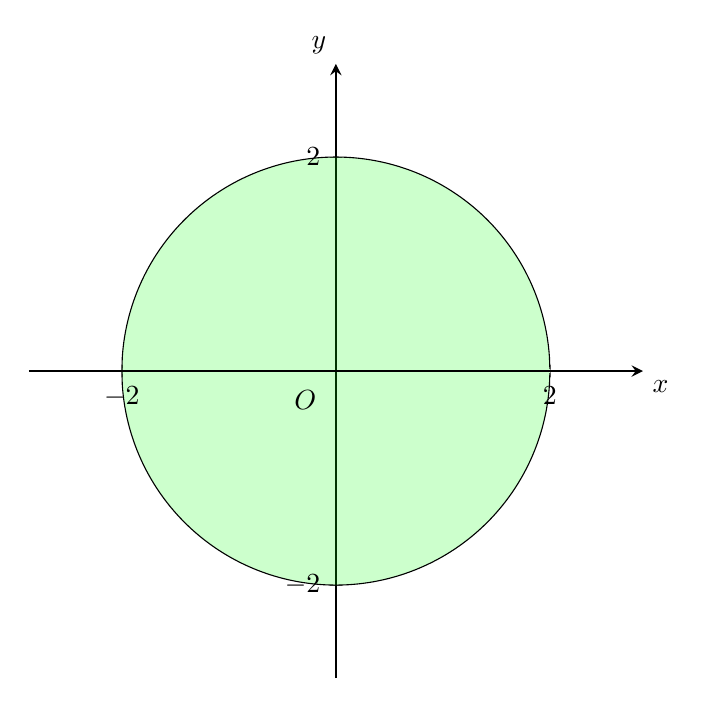
\begin{tikzpicture}
    \begin{axis}[standard,
            xtick={-2.718,2.718},
            ytick={-2.718,2.718},
            samples=1000,
            xlabel={$x$},
            ylabel={$y$},
            xmin=-3,xmax=3,
            ymin=-3,ymax=3,
            x=1cm,
            y=1cm/1,
            xticklabels={$-2$,$2$},
            yticklabels={$-2$,$2$}
           ]
\node[anchor=center,label=south west:$O$] at (axis cs:0,0){};
\addplot[name path=F,domain={-2.718:2.718}]{sqrt(2.718^2-x^2};
\addplot[name path=G,domain={-2.718:2.718}]{-sqrt(2.718^2-x^2};
\addplot[name path=H,domain={-2.718:2.718}]{0};
\addplot[fill=green, fill opacity=0.2] fill between [of=F and H, soft clip={domain=-2.718:2.718}];
\addplot[fill=green, fill opacity=0.2] fill between [of=G and H, soft clip={domain=-2.718:2.718}];
    \end{axis}
    \end{tikzpicture}
}
\end{center}
A circle of radius $2$... let's use polar!

Let's find the bounds for $r$ and $\theta$.

Our lower and upper bounds for $r$ are $r=0$ and $r=2$, respectively.

Our lower and upper bounds for $t$ are $t=0$ and $t=2\pi$, respectively.

In polar,
\begin{align*}
    2x&=2r\cos\theta\tag{$x=r\cos \theta$}\\
    2y&=2r\sin\theta\tag{$y=r\sin\theta$}\\
    \implies 2x - 2y &= 2r\cos\theta - 2r\sin\theta
\end{align*}
Let's evaluate the integral.
\begin{align*}
    \int_C y^2\,dx+x^2\,dy&=\int_0^{2\pi}\int_0^2\lrp{2r\cos\theta-2r\sin\theta}r\,dr\,d\theta\\
    &=\int_0^{2\pi}\int_0^2 2r^2\cos\theta-2r^2\sin\theta\,dr\,d\theta\\
    &=\int_0^{2\pi}\lrb{\frac{2}{3}r^3\cos\theta-\frac{2}{3}r^3\sin\theta}_0^2\,d\theta\\
    &=\int_0^{2\pi}\frac{2}{3}(2)^3\cos\theta-\frac{2}{3}(2)^3\sin\theta\,d\theta\\
    &=\frac{2}{3}(2)^3\int_0^{2\pi}\cos\theta-\sin\theta\,d\theta\tag{we can take constants out}\\
    &=\frac{2}{3}(2)^3\lrb{\sin \theta+\cos\theta}_0^{2\pi}\\
    &=\frac{2}{3}(2)^3\Big(\lrp{\sin 2\pi+\cos 2\pi}-\lrp{\sin 0+\cos 0}\Big)\\
    &=\frac{2}{3}(2)^3 \Big(\lrp{0+1}-\lrp{0+1}\Big)\\
    &=\frac{2}{3}(2)^3\lrp{1-1}\\
    &=\boxed{0}
\end{align*}
\textbf{Note}

You could have also evaluated this integral directly using $\r(t)=\lra{2\cos t, 2\sin t}$.

\phantomsection
\addcontentsline{toc}{section}{Problem 9}\textbf{Problem 9}

Determine whether the vector field $\F(x,y,z)=\dfrac{\lra{1,z,y}}{x+yz}$ is conservative.

\Solution

\phantomsection
\addcontentsline{toc}{subsection}{Potential Function}\textbf{Potential Function Method}

Recall that if a vector field is conservative, then there exists a potential function $f$ for it.

It looks like $\displaystyle f=\ln(x+yz)$ when $x+yz>0$ and $\displaystyle f=\ln(-x-yz)$ when $x+yz<0$. We can verify this by checking if $\nabla f =\F$.

When $\displaystyle f=\ln(x+yz)$,
\begin{align*}
    \nabla f &=\lra{\frac{1}{x+yz},\frac{z}{x+yz},\frac{y}{x+yz}}\\
    &=\frac{\lra{1,z,y}}{x+yz}\\
    &=\F
\end{align*}
When $\displaystyle f=\ln(-x-yz)$,
\begin{align*}
    \nabla f &=\lra{-\frac{1}{-x-yz},\frac{-z}{-x-yz},\frac{-y}{-x-yz}}\\
    &=\lra{\frac{-1}{-(x+yz)},\frac{-z}{-(x+yz)},\frac{-y}{-(x+yz)}}\\
    &=\lra{\frac{1}{x+yz},\frac{z}{x+yz},\frac{y}{x+yz}}\\
    &=\frac{\lra{1,z,y}}{x+yz}\\
    &=\F
\end{align*}
Since potential functions for $\F$ exists, $\F$ is conservative.

\qed

\phantomsection
\addcontentsline{toc}{subsection}{Component Test Method}\textbf{Component Test Method}

Recall that if a vector field is conservative,
\begin{align*}
    \frac{\partial M}{\partial y}=\frac{\partial N}{\partial x},\hspace{2em}\frac{\partial M}{\partial z}=\frac{\partial P}{\partial x},\hspace{2em} \text{and}\hspace{2em}\frac{\partial N}{\partial z}=\frac{\partial P}{\partial y}.
\end{align*}
Since $\F(x,y,z)=\dfrac{\lra{1,z,y}}{x+yz}$,
\begin{align*}
    M&=\frac{1}{x+yz}\\
    N&=\frac{z}{x+yz}\\
    P&=\frac{y}{x+yz}
\end{align*}
Let's check if $\F$ is conservative.
\phantomsection
\addcontentsline{toc}{subsection}{M and N}
For $\displaystyle \frac{\partial M}{\partial y}$ and $\displaystyle \frac{\partial N}{\partial x}$,
\begin{align*}
    \frac{\partial M}{\partial y}&=\frac{0(x+yz)-z(1)}{(x+yz)^2}=\frac{-z}{(x+yz)^2}\\
    \frac{\partial N}{\partial x}&=\frac{0(x+yz)-(1)(z)}{(x+yz)^2}=\frac{-z}{(x+yz)^2}
\end{align*}
Therefore, $\displaystyle \frac{\partial M}{\partial y}=\frac{-z}{(x+yz)^2}= \frac{\partial N}{\partial x}$.

\phantomsection
\addcontentsline{toc}{subsection}{M and P}
For $\displaystyle \frac{\partial M}{\partial z}$ and $\displaystyle\frac{\partial P}{\partial x}$,
\begin{align*}
    \frac{\partial M}{\partial z}&=\frac{0(x+yz)-y(1)}{(x+yz)^2}=\frac{-y}{(x+yz)^2}\\
    \frac{\partial P}{\partial x}&=\frac{0(x+yz)-(1)(y)}{(x+yz)^2}=\frac{-y}{(x+yz)^2}
\end{align*}
Therefore, $\displaystyle \frac{\partial M}{\partial z}=\frac{-y}{(x+yz)^2}=\frac{\partial P}{\partial x}$.

\phantomsection
\addcontentsline{toc}{subsection}{N and P}
For $\displaystyle \frac{\partial N}{\partial z}$ and $\displaystyle\frac{\partial P}{\partial y}$,
\begin{align*}
    \frac{\partial N}{\partial z}&=\frac{1(x+yz)-y(z)}{(x+yz)^2}=\frac{x+yz-yz}{(x+yz)^2}=\frac{x}{(x+yz)^2}\\
    \frac{\partial P}{\partial y}&=\frac{1(x+yz)-z(y)}{(x+yz)^2}=\frac{x+yz-yz}{(x+yz)^2}=\frac{x}{(x+yz)^2}
\end{align*}
Therefore, $\displaystyle \frac{\partial N}{\partial z}=\frac{x}{(x+yz)^2}=\frac{\partial P}{\partial y}$.

Since $\displaystyle \frac{\partial M}{\partial y}=\frac{\partial N}{\partial x}$, $\displaystyle \frac{\partial M}{\partial z}=\frac{\partial P}{\partial x}$, and $\displaystyle \frac{\partial N}{\partial z}=\frac{\partial P}{\partial y}$, $\F$ is conservative.

\qed

\newpage
\phantomsection
\addcontentsline{toc}{section}{Problem 10}\textbf{Problem 10}

Find a potential function for the vector field $\F(x,y,z)=\lra{z\cos xz,e^y,x\cos xz}$.

\Solution

\textbf{Note}

Note that we're just looking for \textit{a} potential function, not a \textit{general} potential function. For this reason, we're going to assume $C=0$. No more $+C$ integral horror stories here...

We can either do the ``guess and check" method or the formal method.

\phantomsection
\addcontentsline{toc}{subsection}{Guess And Check Method}\textbf{Guess And Check Method}

It looks like $f(x,y,z)=\sin xz + e^y$. We can verify this by checking if $\nabla f(x,y,z)=\F$.
\begin{align*}
    \nabla f(x,y,z)&=\lra{\frac{\partial f}{\partial x}, \frac{\partial f}{\partial y}, \frac{\partial f}{\partial z}}\\
    &=\lra{z\cos xz, e^y, x\cos xz}\\
    &=\F
\end{align*}
Since $\nabla f(x,y,z)=\F$,
\begin{equation*}
    \boxed{f(x,y,z)=\sin xz+e^y}
\end{equation*}

\phantomsection
\addcontentsline{toc}{subsection}{Formal Method}\textbf{Formal Method}

If $\F$ is conservative, then there exists a potential function $f$.

Recall that $\F$ is conservative if and only if
\begin{align*}
    \frac{\partial M}{\partial y}=\frac{\partial N}{\partial x},\hspace{2em}\frac{\partial M}{\partial z}=\frac{\partial P}{\partial x},\hspace{2em} \text{and}\hspace{2em}\frac{\partial N}{\partial z}=\frac{\partial P}{\partial y}.
\end{align*}
Let's check if $\F$ is conservative.

\phantomsection
\addcontentsline{toc}{subsubsection}{M and N}
For $\displaystyle \frac{\partial M}{\partial y}$ and $\displaystyle \frac{\partial N}{\partial x}$,
\begin{align*}
    \frac{\partial M}{\partial y}&=0\\
    \frac{\partial N}{\partial x}&=0
\end{align*}
Therefore, $\displaystyle \frac{\partial M}{\partial y}=0= \frac{\partial N}{\partial x}$.

\phantomsection
\addcontentsline{toc}{subsubsection}{M and P}
For $\displaystyle \frac{\partial M}{\partial z}$ and $\displaystyle\frac{\partial P}{\partial x}$,
\begin{align*}
    \frac{\partial M}{\partial z}&=-xz\sin xz\\
    \frac{\partial P}{\partial x}&=-xz\sin xz
\end{align*}
Therefore, $\displaystyle \frac{\partial M}{\partial z}=-xz\sin xz=\frac{\partial P}{\partial x}$.

\phantomsection
\addcontentsline{toc}{subsubsection}{N and P}
For $\displaystyle \frac{\partial N}{\partial z}$ and $\displaystyle\frac{\partial P}{\partial y}$,
\begin{align*}
    \frac{\partial N}{\partial z}&=0\\
    \frac{\partial P}{\partial y}&=0
\end{align*}
Therefore, $\displaystyle \frac{\partial N}{\partial z}=0=\frac{\partial P}{\partial y}$.

Since $\displaystyle \frac{\partial M}{\partial y}=\frac{\partial N}{\partial x}$, $\displaystyle \frac{\partial M}{\partial z}=\frac{\partial P}{\partial x}$, and $\displaystyle \frac{\partial N}{\partial z}=\frac{\partial P}{\partial y}$, $\F$ is conservative.

Since $\F$ is conservative, let's start finding it's potential function.

Since $\displaystyle \frac{\partial f}{\partial x}=z\cos xz$,
\begin{align*}
    f(x,y,z)&=\sin xz +g(y,z)
\end{align*}
Since $\displaystyle \frac{\partial f}{\partial y}=e^y$,
\begin{align*}
    \frac{\partial f}{\partial y}=0+\frac{\partial g}{\partial y}&=e^y\\
    \implies \frac{\partial g}{\partial y}&=e^y\\
    \implies f(x,y,z)&=\sin xz + e^y+h(z)
\end{align*}
Since $\displaystyle \frac{\partial f}{\partial z}=x\cos xz$,
\begin{align*}
    \frac{\partial f}{\partial z}=x\cos xz + 0 +\frac{\partial h}{\partial z}&=x\cos xz\\
    \implies \frac{\partial h}{\partial z}&=0\\
    \implies f(x,y,z)&=\sin xz + e^y\tag{let $C=0$ aka ignore $C$}
\end{align*}
Therefore,
\begin{equation*}
    \boxed{f(x,y,z)=\sin xz+e^y}
\end{equation*}
\phantomsection
\addcontentsline{toc}{section}{Problem 11}\textbf{Problem 11}

Find the work done by $\F(x,y)=\dfrac{\lra{x,y}}{(x^2+y^2)^{3/2}}$ over the curve $\r(t)=\lra{e^t\cos t,e^t\sin t}$ from $(1,0)$ to $\lrp{e^{2\pi},0}$ both directly and using a potential function.

\Solution

\phantomsection
\addcontentsline{toc}{subsection}{Direct Method} \textbf{Direct Method}

Recall that work done by the force $\F$ over a curve is
\begin{align*}
    W&=\int_C M\,dx + N\,dy + P\,dz=\int_a^b \F\lrp{\r(t)}\cdot d\r
\end{align*}
Note that this is \textit{one} of the many ways to define work. I am using the definition of work that is convenient for this problem. Plus, remembering the formula this way helps you remember the other identical formulas hahaha

If we're going from $(1,0)$ to $\lrp{e^{2\pi},0}$, then $0\leq t\leq 2\pi$. This makes sense because at $t=0$, $\r(0)=\lra{e^0\cos 0, e^0\sin 0}=\lra{1, 0}$ and at $t=2\pi$, $\r(2\pi)=\lra{e^{2\pi}\cos 2\pi, e^{2\pi}\sin 2\pi}=\lra{e^{2\pi},0}$.

If $\r(t)=\lra{e^t\cos t,e^t\sin t}$, then
\begin{align*}
    \F\lrp{\r(t)}&=\frac{\lra{e^t\cos t,e^t\sin t}}{\Big(\lrp{e^t\cos t}^2+\lrp{e^t\sin t}^2\Big)^{3/2}}\\
    &=\frac{\lra{e^t\cos t,e^t\sin t}}{\lrp{e^{2t}\cos^2t + e^{2t}\sin ^2 t}^{3/2}}\\
    &=\frac{\lra{e^t\cos t,e^t\sin t}}{\lrp{e^{2t}(\cos^2t +\sin^2t}^{3/2}}\\
    &=\frac{\lra{e^t\cos t,e^t\sin t}}{\lrp{e^{2t}}^{3/2}}\tag{$\cos^2 t+\sin^2 t=1$}\\
    &=\frac{\lra{e^t\cos t,e^t\sin t}}{e^{3t}}\tag{$\lrp{e^{2t}}^{3/2}=e^{\frac{6t}{2}}=e^{3t}$}\\
    &=\lra{e^{-2t}\cos t, e^{-2t}\sin t}\tag{$\frac{e^t}{e^{3t}}=e^{t-3t}=e^{-2t}$}\\
    \r'(t)&=\lra{e^t\cos t - e^t\sin t, e^t\sin t + e^t \cos t}
\end{align*}
Let's evaluate the work integral.
\begin{align*}
    \text{work}&=\int_0^{2\pi}\lra{e^{-2t}\cos t, e^{-2t}\sin t}\cdot\lra{e^t\cos t - e^t\sin t, e^t\sin t + e^t \cos t}\,dt\\
    &=\int_0^{2\pi}\lrp{e^{-2t}\cos t}\lrp{e^t\cos t-e^t\sin t}+\lrp{e^{-2t}\sin t}\lrp{e^t\sin t+e^t\cos t}\,dt\\
    &=\int_0^{2\pi} \lrp{e^{-t}\cos^2 t-e^{-t}\sin t\cos t}+\lrp{e^{-t}\sin^2 t+e^{-t}\sin t\cos t}\, dt\tag{$e^{-2t}e^t=e^{-2t+t}=e^{-t}$}\\
    &=\int_0^{2\pi} e^{-t}\cos^2 t + e^{-t}\sin ^2 t\,dt\\
    &=\int_0^{2\pi} e^{-t}\lrp{\cos ^2 t+\sin ^2 t}\,dt\\
    &=\int_0^{2\pi} e^{-t}\,dt\tag{$\cos ^2 t + \sin ^2 t =1$}\\
    &=\lrb{-e^{-t}}_0^{2\pi}\\
    &=\lrp{-e^{-2\pi}}-\lrp{-e^{-0}}\\
    &=-e^{-2\pi}-\lrp{-1}\tag{$e^0=1$}\\
    &=\boxed{-e^{-2\pi}+1}
\end{align*}

\phantomsection
\addcontentsline{toc}{subsection}{Potential Function} \textbf{Potential Function}

If we can find a potential function for $\F$, then
\begin{equation*}
    \text{work}=\int_a^b \F\lrp{\r(t)}\cdot d\r=\lrb{f\lrp{\r(t)}}_a^b
\end{equation*}
Since the problem is asking us to use a potential function, we're going to assume that a potential function actually exists.

Since $\displaystyle\frac{\partial f}{\partial x}=\frac{x}{(x^2+y^2)^{3/2}}$,
\begin{align*}
    f(x,y)&=-(x^2+y^2)^{-1/2}+h(y)\tag{you can verify this yourself}
\end{align*}
Since $\displaystyle\frac{\partial f}{\partial y}=\frac{y}{(x^2+y^2)^{3/2}}$,
\begin{align*}
    \frac{\partial f}{\partial y}=\frac{1}{2}\lrp{x^2+y^2}^{-3/2}\lrp{2y}=\frac{y}{\lrp{x^2+y^2}^{3/2}}+\frac{\partial  h}{\partial y}&=\frac{y}{(x^2+y^2)^{3/2}}\\
    \implies \frac{\partial h}{\partial y}&=0\\
    \implies f(x,y)&=-\lrp{x^2+y^2}^{-1/2}\tag{let $C=0$ aka ignore $C$}
\end{align*}
Let's evaluate the work integral.
\begin{align*}
    \text{work}&=\int_C \F\cdot d\r\\
    &=\lrb{f(x,y)}_{(1,0)}^{(e^{2\pi},0)}\\
    &=f(e^{2\pi},0)-f(1,0)\\
    &=\lrp{-\Big(\lrp{e^{2\pi}}^2+0^2\Big)^{-1/2}}-\lrp{-\Big(1^2+0^2\Big)^{-1/2}}\\
    &=\lrp{-\lrp{e^{4\pi}}^{-1/2}}-\lrp{-\lrp{1}^{-1/2}}\\
    &=-e^{-2\pi}-\lrp{-1}\\
    &=\boxed{-e^{-2\pi}+1}
\end{align*}

\phantomsection
\addcontentsline{toc}{section}{Problem 12}\textbf{Problem 12}

Find the circulation and flux for the field $\F(x,y)=\lra{y-6x^2,x+y^2}$ around and across the triangle given by $y=0$, $y=x$, and $x=1$.

\Solution

\phantomsection
\addcontentsline{toc}{subsection}{Circulation}\textbf{Circulation}

Recall that circulation for a vector field $\F$ around and across a curve $C$ is
\begin{equation*}
    \text{circulation}= \iint_R \frac{\partial N}{\partial x} - \frac{\partial M}{\partial y}\,dA
\end{equation*}
If $\F(x,y)=\lra{y-6x^2,x+y^2}$, then
\begin{align*}
    M=y-6x^2&\implies \frac{\partial M}{\partial y}= 1\\
    N=x+y^2&\implies \frac{\partial N}{\partial x}= 1
\end{align*}
To find our region $R$, let's graph the triangle given by $y=0$, $y=x$, and $x=1$.
\begin{center}
\resizebox{3.5cm}{!}{
    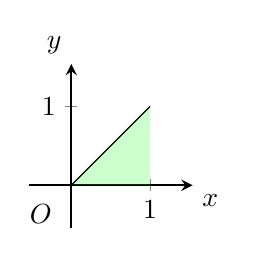
\begin{tikzpicture}
    \begin{axis}[standard,
            xtick={1},
            ytick={1},
            samples=1000,
            xlabel={$x$},
            ylabel={$y$},
            xmin=-0.3,xmax=1.3,
            ymin=-.3,ymax=1.3,
            x=1cm,
            y=1cm/1,
           ]
\node[anchor=center,label=south west:$O$] at (axis cs:0,0){};
\addplot[name path=F,domain={0:1}]{x};
\addplot[name path=G,domain={0:1}]{0};
\addplot[fill=green, fill opacity=0.2] fill between [of=F and G, soft clip={domain=0:1}];
    \end{axis}
    \end{tikzpicture}
}
\end{center}
Our lower and upper bounds for $y$ are $y=0$ and $y=x$, respectively.

Our lower and upper bounds for $x$ are $x=0$ and $x=1$, respectively.

Let's evaluate the circulation integral.
\begin{align*}
    \text{circulation}&=\int_0^1\int_0^x 1 - 1 \,dy\,dx\\
    &=\int_0^1\int_0^x 0\,dy\,dx\\
    &=\int_0^1 0\,dx\tag{integral of $0$ is $0$}\\
    &=0\tag{integral of $0$ is $0$}
\end{align*}

\phantomsection
\addcontentsline{toc}{subsection}{Flux}\textbf{Flux}

Recall that flux for a vector field around and across a curve $C$ is
\begin{equation*}
   \text{flux} = \iint_R \frac{\partial M}{\partial x} + \frac{\partial N}{\partial y}\,dA
\end{equation*}
If $\F(x,y)=\lra{y-6x^2,x+y^2}$, then
\begin{align*}
     M=y-6x^2&\implies \frac{\partial M}{\partial x}=-12x\\
    N=x+y^2&\implies \frac{\partial N}{\partial y}= 2y
\end{align*}
Our region $R$ for flux is going to be the same as our region $R$ for circulation. Therefore, the flux bounds for
$x$ and $y$ are the same as the circulation bounds for $x$ and $y$.

Let's evaluate the flux integral.
\begin{align*}
    \text{flux}&=\int_0^1 \int_0^x -12x + 2y\,dy\,dx\\
    &=\int_0^1 \lrb{-12xy+y^2}_0^x\,dx\\
    &=\int_0^1 -12x^2 + x^2\,dx\\
    &=\int_0^1 -11x^2\,dx\\
    &=\lrb{-\frac{11}{3}x^3}_0^1\\
    &=-\frac{11}{3}
\end{align*}
Our final answer is
\begin{subequations}
    \begin{empheq}[box=\widefbox]{align}
      \text{circulation}&=0\nonumber\\
      \text{flux}&=-\frac{11}{3}\nonumber
    \end{empheq}
\end{subequations}

\newpage
\phantomsection
\addcontentsline{toc}{section}{Problem 13}\textbf{Problem 13}

Show that the radius of curvature of a plane curve $\r(t)=\lra{x(t),y(t)}$ is given by
\begin{equation*}
    \rho(t)=\frac{x'(t)^2+y'(t)^2}{\sqrt{x''(t)^2+y''(t)^2-s''(t)^2}}
\end{equation*}
where $\displaystyle s''(t)=\frac{d}{dt}\sqrt{x'(t)^2+y'(t)^2}$.

\Solution

Recall that the curvature of $\r(t)=\lra{x(t),y(t)}$ is
\begin{align*}
    \kappa=\frac{\left|x'y''-y'x''\right|}{((x')^2+(y')^2)^{3/2}}
\end{align*}
(Homework 9, 2(d); Campuswire \#45)

Recall that the radius of curvature is
\begin{align*}
    \rho=\frac{1}{\kappa}=\frac{((x')^2+(y')^2)^{3/2}}{\left|x'y''-y'x''\right|}
\end{align*}
If $\displaystyle s''(t)=\frac{d}{dt}\sqrt{x'(t)^2+y'(t)^2}$, then
\begin{align*}
    s''&=\frac{1}{2\big((x')^2+(y')^2\big)^{1/2}}\big(2x'x''+2y'y''\big)=\frac{x'x''+y'y''}{\big((x')^2+(y')^2\big)^{1/2}}\\
    \lrp{s''}^2&=\lrp{\frac{x'x''+y'y''}{\big((x')^2+(y')^2\big)^{1/2}}}^2=\frac{\lrp{x'}^2\lrp{x''}^2+2x'x''y'y''+\lrp{y'}^2\lrp{y''}^2}{(x')^2+(y')^2}\\
    \lrp{x''}^2+\lrp{y''}^2-\lrp{s''}^2&= \lrp{x''}^2+\lrp{y''}^2-\frac{\lrp{x'}^2\lrp{x''}^2+2x'x''y'y''+\lrp{y'}^2\lrp{y''}^2}{(x')^2+(y')^2}\\
    &=\frac{\lrp{x''}^2\lrp{(x')^2+(y')^2}}{(x')^2+(y')^2}+\frac{\lrp{y''}^2\lrp{(x')^2+(y')^2}}{(x')^2+(y')^2}-\frac{\lrp{x'}^2\lrp{x''}^2+2x'x''y'y''+\lrp{y'}^2\lrp{y''}^2}{(x')^2+(y')^2}\\
    &=\frac{\lrp{x'}^2\lrp{x''}^2+\lrp{x''}^2\lrp{y'}^2}{(x')^2+(y')^2}+\frac{\lrp{x'}^2\lrp{y''}^2+\lrp{y'}^2\lrp{y''}^2}{(x')^2+(y')^2}-\frac{\lrp{x'}^2\lrp{x''}^2+2x'x''y'y''+\lrp{y'}^2\lrp{y''}^2}{(x')^2+(y')^2}\\
    &=\frac{\lrp{x''}^2\lrp{y'}^2+\lrp{x'}^2\lrp{y''}^2-2x'x''y'y''}{\lrp{x'}^2+\lrp{y'}^2}\\
    &=\frac{\lrp{x'}^2\lrp{y''}^2-2x'x''y'y''+\lrp{x''}^2\lrp{y'}^2}{\lrp{x'}^2+\lrp{y'}^2}\\
    &=\frac{\lrp{x'y''-y'y''}^2}{\lrp{x'}^2+\lrp{y'}^2}\tag{factor}
\end{align*}
Since $\displaystyle \lrp{x''}^2+\lrp{y''}^2-\lrp{s''}^2=\frac{\lrp{x'y''-y'y''}^2}{\lrp{x'}^2+\lrp{y'}^2}$,
\begin{align*}
    \sqrt{\lrp{x''}^2+\lrp{y''}^2-\lrp{s''}^2}&=\frac{\left|x'y''-y'x''\right|}{\big(\lrp{x'}^2+\lrp{y'}^2\big)^{1/2}}\\
    \implies \big(\lrp{x'}^2+\lrp{y'}^2\big)^{1/2}\sqrt{\lrp{x''}^2+\lrp{y''}^2-\lrp{s''}^2}&=\left|x'y''-y'x''\right|
\end{align*}
Since $\displaystyle \left|x'y''-y'x''\right|=\big(\lrp{x'}^2+\lrp{y'}^2\big)^{1/2}\sqrt{\lrp{x''}^2+\lrp{y''}^2-\lrp{s''}^2}$,
\begin{align*}
    \rho(t)=\frac{1}{\kappa}&=\frac{((x')^2+(y')^2)^{3/2}}{\left|x'y''-y'x''\right|}\tag{recall from above}\\
    &=\frac{((x')^2+(y')^2)^{3/2}}{\big(\lrp{x'}^2+\lrp{y'}^2\big)^{1/2}\sqrt{\lrp{x''}^2+\lrp{y''}^2-\lrp{s''}^2}}\\
    &=\frac{x'(t)^2+y'(t)^2}{\sqrt{x''(t)^2+y''(t)^2-s''(t)^2}}\tag{adding the $(t)$ for notational fluff}
\end{align*}
\qed
\end{document}
